\section{Experiments}
\label{sec:experiments}

Say you are hosting an elegant dinner party, and wish to select a balanced set of wines for drinking and flowers for decoration.
We demonstrate \tsip~ and \greedy~ on the Iris and Wine datasets \citep{misc_iris_53, misc_wine_109, scikit-learn}.
This has an intuitive interpretation as selecting diverse elements that reflects the peculiar structure of the diversification problem.
Features like \textit{ petal width} are rows in $X$.
They are features on the basis of which we may select among the flowers those which are most distinct from another.
Thus, in diversification, $P = n$.

We also analyze the Ethanol dataset from \citet{Chmiela2018-at, Koelle2022-ju}, but rather than selecting between bourbon and scotch we evaluate a dictionary of interpretable features  - bond torsions - for their ability to parameterize the molecular configuration space.
In this interpretability use case, columns denote gradients of informative features.
We compute Jacoban matrices of putative parametrization functions and project them onto estimated tangent spaces (see \citet{Koelle2022-ju} for preprocessing details).
Rather than selecting between data points, we are selecting between functions which parameterize the data.

For basis pursuit, we use the SCS interior point solver \citep{ocpb:16} from CVXPY \citep{diamond2016cvxpy, agrawal2018rewriting}, which is able to push sparse values arbitrarily close to 0 \citep{cvxpy_sparse_solution}.
Statistical replicas for Wine and Iris are created by resampling across $[P]$.
Due to differences in scales between rows, these are first standardized.
For the Wine dataset, even \brute~ on $\widehat {S}_{IP}$ is prohibitive in $D=13$, and so we truncate our inputs to $D=6$.
For Ethanol, replicas are created by sampling from data points and their corresponding tangent spaces are estimated in $B = 252$.

Figure \ref{fig:isometry_losses} and Table \ref{tab:experiments} show that the $l_1$ accrued by the subset $\widehat S_{G}$ estimated using \greedy~ with objective $l_1$ is higher than that for the subset estimated by \tsip.
This effect is statistically significant, but varies across datapoints and datasets.
Figure \ref{fig:support_cardinalities} details intermediate support recovery cardinalities from \isometrypursuit.
We also evaluated second stage \brute~ selection after random selection of $\widehat S_{IP}$ but do not report it since it often lead to catastrophic failure to satisfy the basis pursuit constraint.
Wall-clock runtimes are given in Section \ref{sec:timing}.

\begin{table}[h!]
\tiny
\centering
\begin{tabular}{|c|c|c|c|c|c|c|c|c|c|c|}
\toprule
Name & $D$ & $P$ & $R$ & $c$ & $l_1(X_{.\widehat{S}_{G}})$ & $|\widehat{S}_{IP}|$ & $l_1(X_{.\widehat{S}})$ & $\thead{\tiny P_R (l_1(X_{.\widehat{S}_{G}})  \\ > l_1(X_{.\widehat{S}_{}}))}$ & $ \thead{ \tiny P_R (l_1(X_{.\widehat{S}_{G}}) \\ = l_1(X_{.\widehat{S}_{}}))}$ & $\thead{ \tiny \widehat P(\bar{l}_1(X_{.\widehat{S}_{G}}) \\> \bar{l}_1(X_{.\widehat{S}_{}}))}$ \\
\midrule
Iris & 4 & 75 & 25 & 1 & 13.8 ± 7.3 & 7 ± 1 & 6.9 ± 1.4 & 0.96 & 0. & 2.4e-05 \\
Wine & 6 & 89 & 25 & 1 & 7.7 ± 0.3 & 13 ± 2 & 7.6 ± 0.3 & 0.64 & 0.16 & 6.3e-04 \\
Ethanol & 2 & 756 & 100 & 1 & 2.6 ± 0.3 & 90 ± 165 & 2.5 ± 0.2 & 0.66 & 0.17 & 2.1e-05 \\
\bottomrule
\end{tabular}
\caption{Experimental parameters and results.
For Iris and Wine, $P$ results from random downsampling by a factor of $2$ to create $R$ replicates.
$P_R$ values are empirical probabilities, while estimated P-values $\widehat P$ are computed by paired two-sample T-test on  $l_1(X_{.\widehat S})$ and $l_1(X_{.\widehat S_{G}})$.
For brevity, in this table $\widehat S := \widehat {S}_{TSIP}$.
}
\label{tab:experiments}
\end{table}

\begin{figure}[t]
    \centering
    % Subfigure for Wine dataset
    \begin{subfigure}[b]{0.3\textwidth}
        \centering
        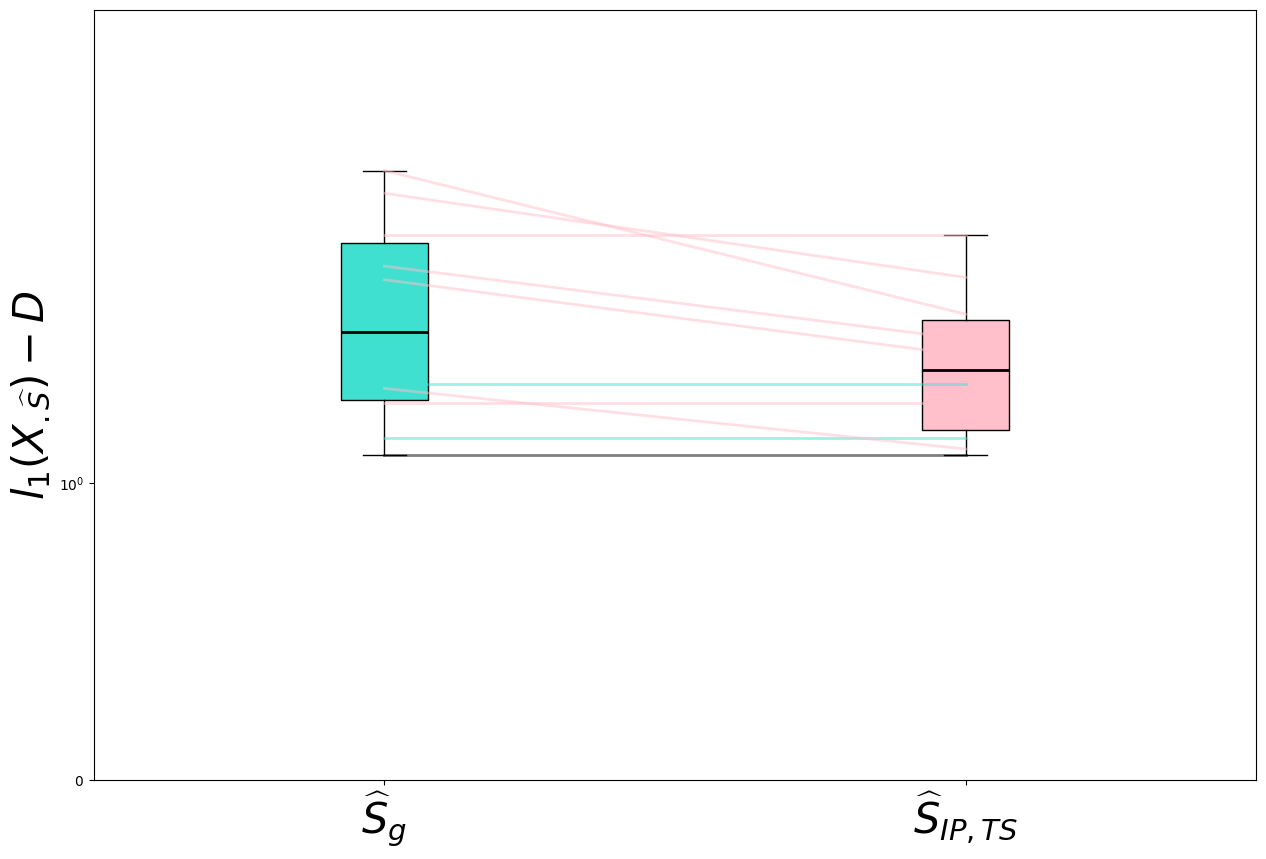
\includegraphics[width=\textwidth]{../figures/wine_standardized_0p5_1p0_isometry_losses}
        \caption{Wine dataset}
        \label{fig:wine_isometry_losses}
    \end{subfigure}
    \hfill
    % Subfigure for Iris dataset
    \begin{subfigure}[b]{0.3\textwidth}
        \centering
        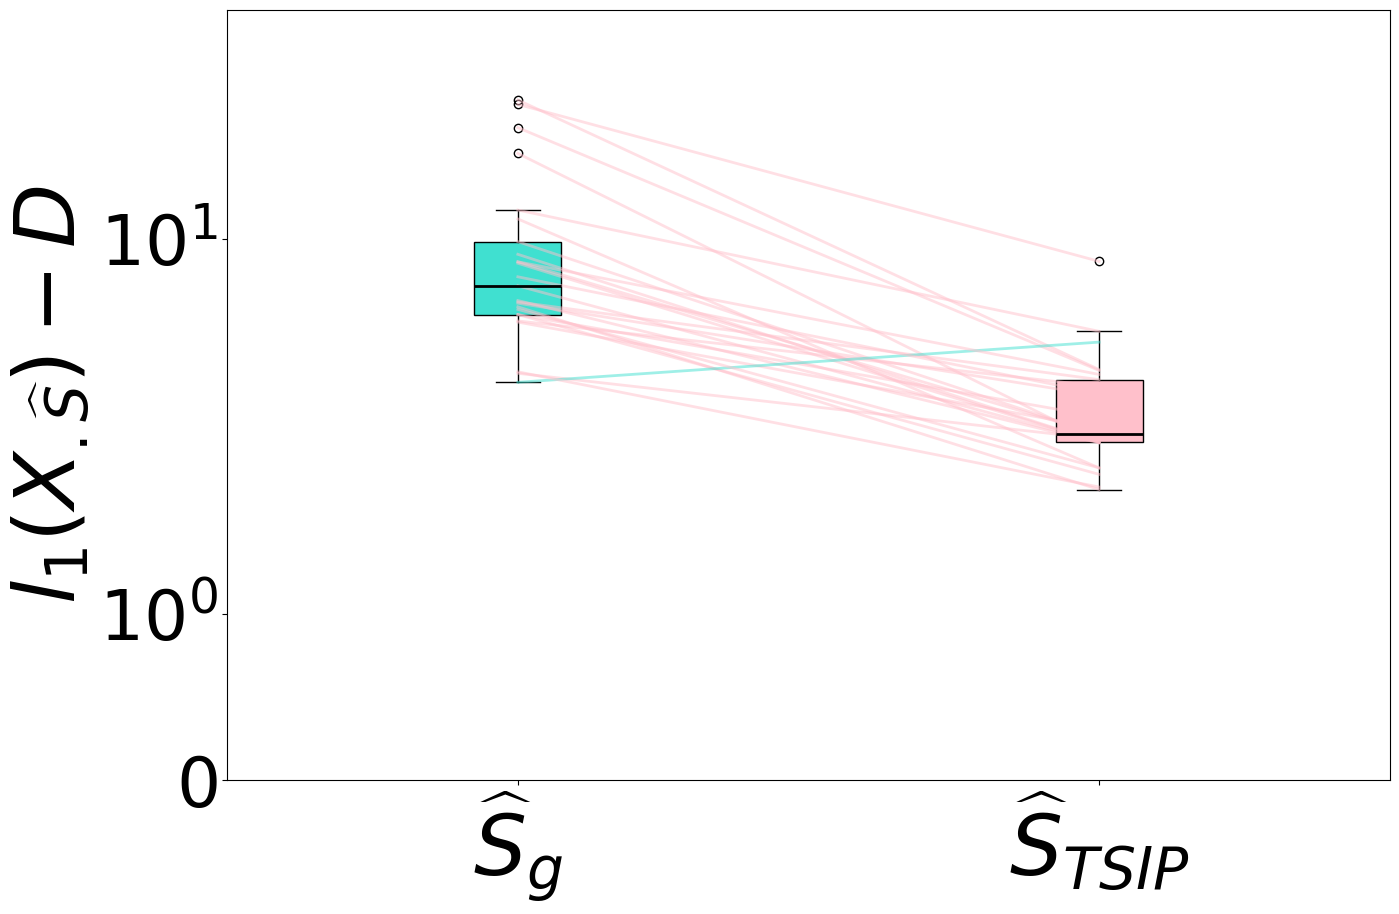
\includegraphics[width=\textwidth]{../figures/iris_standardized_0p5_1p0_isometry_losses}
        \caption{Iris dataset}
        \label{fig:iris_isometry_losses}
    \end{subfigure}
    \hfill
    % Subfigure for Ethanol dataset
    \begin{subfigure}[b]{0.3\textwidth}
        \centering
        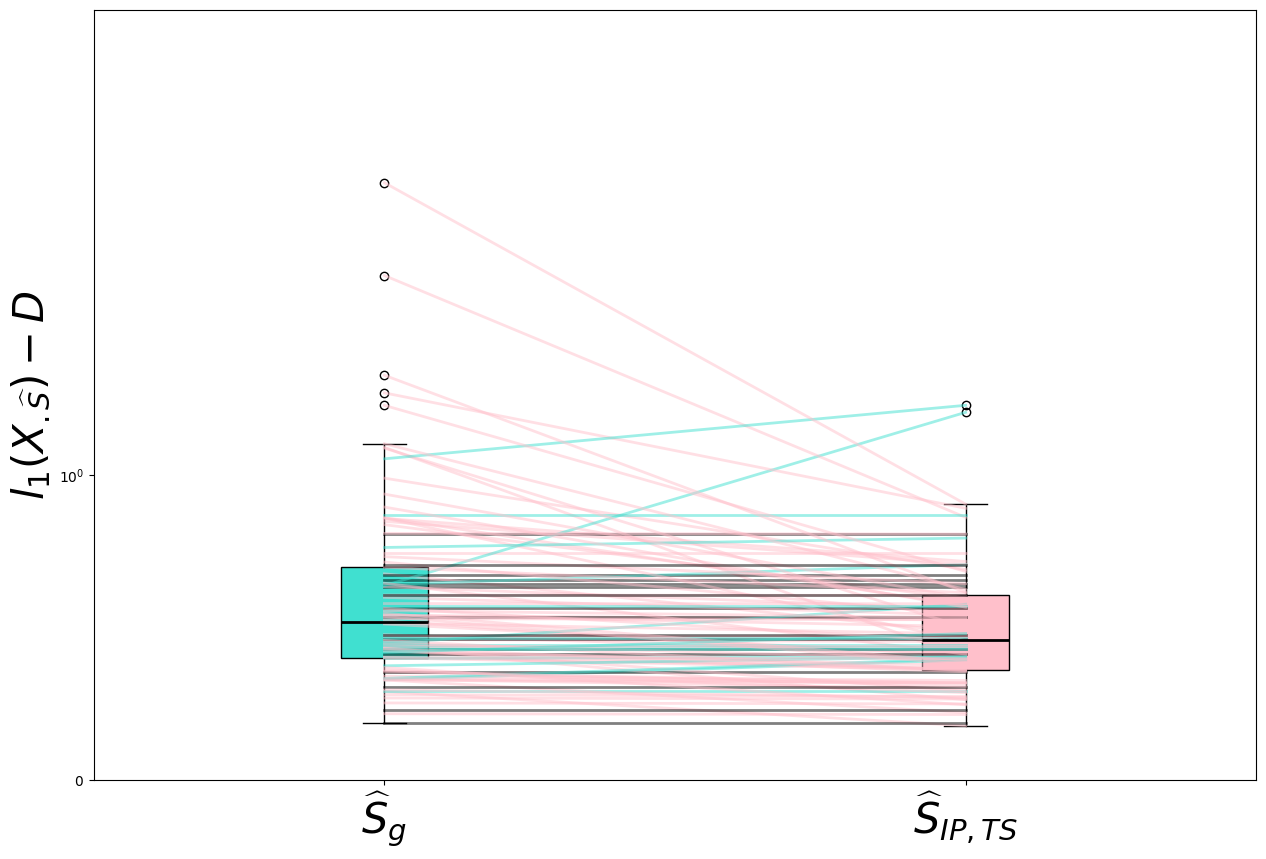
\includegraphics[width=\textwidth]{../figures/ethanol_isometry_losses}
        \caption{Ethanol dataset}
        \label{fig:ethanol_isometry_losses}
    \end{subfigure}
    \caption{Isometry losses $l_1$  for Wine, Iris, and Ethanol datasets across $R$ replicates.
    Lower greedy losses are shown with turquoise, while lower two stage losses are shown with pink.
    Equal losses are shown with black lines.
    As detailed in Table \ref{tab:experiments}, losses are generally lower for two-stage isometry pursuit solutions.}
    \label{fig:isometry_losses}
\end{figure}
